
% Default to the notebook output style

    


% Inherit from the specified cell style.




    
\documentclass[11pt]{article}

    
    
    \usepackage[T1]{fontenc}
    % Nicer default font (+ math font) than Computer Modern for most use cases
    \usepackage{mathpazo}

    % Basic figure setup, for now with no caption control since it's done
    % automatically by Pandoc (which extracts ![](path) syntax from Markdown).
    \usepackage{graphicx}
    % We will generate all images so they have a width \maxwidth. This means
    % that they will get their normal width if they fit onto the page, but
    % are scaled down if they would overflow the margins.
    \makeatletter
    \def\maxwidth{\ifdim\Gin@nat@width>\linewidth\linewidth
    \else\Gin@nat@width\fi}
    \makeatother
    \let\Oldincludegraphics\includegraphics
    % Set max figure width to be 80% of text width, for now hardcoded.
    \renewcommand{\includegraphics}[1]{\Oldincludegraphics[width=.8\maxwidth]{#1}}
    % Ensure that by default, figures have no caption (until we provide a
    % proper Figure object with a Caption API and a way to capture that
    % in the conversion process - todo).
    \usepackage{caption}
    \DeclareCaptionLabelFormat{nolabel}{}
    \captionsetup{labelformat=nolabel}

    \usepackage{adjustbox} % Used to constrain images to a maximum size 
    \usepackage{xcolor} % Allow colors to be defined
    \usepackage{enumerate} % Needed for markdown enumerations to work
    \usepackage{geometry} % Used to adjust the document margins
    \usepackage{amsmath} % Equations
    \usepackage{amssymb} % Equations
    \usepackage{textcomp} % defines textquotesingle
    % Hack from http://tex.stackexchange.com/a/47451/13684:
    \AtBeginDocument{%
        \def\PYZsq{\textquotesingle}% Upright quotes in Pygmentized code
    }
    \usepackage{upquote} % Upright quotes for verbatim code
    \usepackage{eurosym} % defines \euro
    \usepackage[mathletters]{ucs} % Extended unicode (utf-8) support
    \usepackage[utf8x]{inputenc} % Allow utf-8 characters in the tex document
    \usepackage{fancyvrb} % verbatim replacement that allows latex
    \usepackage{grffile} % extends the file name processing of package graphics 
                         % to support a larger range 
    % The hyperref package gives us a pdf with properly built
    % internal navigation ('pdf bookmarks' for the table of contents,
    % internal cross-reference links, web links for URLs, etc.)
    \usepackage{hyperref}
    \usepackage{longtable} % longtable support required by pandoc >1.10
    \usepackage{booktabs}  % table support for pandoc > 1.12.2
    \usepackage[inline]{enumitem} % IRkernel/repr support (it uses the enumerate* environment)
    \usepackage[normalem]{ulem} % ulem is needed to support strikethroughs (\sout)
                                % normalem makes italics be italics, not underlines
    

    
    
    % Colors for the hyperref package
    \definecolor{urlcolor}{rgb}{0,.145,.698}
    \definecolor{linkcolor}{rgb}{.71,0.21,0.01}
    \definecolor{citecolor}{rgb}{.12,.54,.11}

    % ANSI colors
    \definecolor{ansi-black}{HTML}{3E424D}
    \definecolor{ansi-black-intense}{HTML}{282C36}
    \definecolor{ansi-red}{HTML}{E75C58}
    \definecolor{ansi-red-intense}{HTML}{B22B31}
    \definecolor{ansi-green}{HTML}{00A250}
    \definecolor{ansi-green-intense}{HTML}{007427}
    \definecolor{ansi-yellow}{HTML}{DDB62B}
    \definecolor{ansi-yellow-intense}{HTML}{B27D12}
    \definecolor{ansi-blue}{HTML}{208FFB}
    \definecolor{ansi-blue-intense}{HTML}{0065CA}
    \definecolor{ansi-magenta}{HTML}{D160C4}
    \definecolor{ansi-magenta-intense}{HTML}{A03196}
    \definecolor{ansi-cyan}{HTML}{60C6C8}
    \definecolor{ansi-cyan-intense}{HTML}{258F8F}
    \definecolor{ansi-white}{HTML}{C5C1B4}
    \definecolor{ansi-white-intense}{HTML}{A1A6B2}

    % commands and environments needed by pandoc snippets
    % extracted from the output of `pandoc -s`
    \providecommand{\tightlist}{%
      \setlength{\itemsep}{0pt}\setlength{\parskip}{0pt}}
    \DefineVerbatimEnvironment{Highlighting}{Verbatim}{commandchars=\\\{\}}
    % Add ',fontsize=\small' for more characters per line
    \newenvironment{Shaded}{}{}
    \newcommand{\KeywordTok}[1]{\textcolor[rgb]{0.00,0.44,0.13}{\textbf{{#1}}}}
    \newcommand{\DataTypeTok}[1]{\textcolor[rgb]{0.56,0.13,0.00}{{#1}}}
    \newcommand{\DecValTok}[1]{\textcolor[rgb]{0.25,0.63,0.44}{{#1}}}
    \newcommand{\BaseNTok}[1]{\textcolor[rgb]{0.25,0.63,0.44}{{#1}}}
    \newcommand{\FloatTok}[1]{\textcolor[rgb]{0.25,0.63,0.44}{{#1}}}
    \newcommand{\CharTok}[1]{\textcolor[rgb]{0.25,0.44,0.63}{{#1}}}
    \newcommand{\StringTok}[1]{\textcolor[rgb]{0.25,0.44,0.63}{{#1}}}
    \newcommand{\CommentTok}[1]{\textcolor[rgb]{0.38,0.63,0.69}{\textit{{#1}}}}
    \newcommand{\OtherTok}[1]{\textcolor[rgb]{0.00,0.44,0.13}{{#1}}}
    \newcommand{\AlertTok}[1]{\textcolor[rgb]{1.00,0.00,0.00}{\textbf{{#1}}}}
    \newcommand{\FunctionTok}[1]{\textcolor[rgb]{0.02,0.16,0.49}{{#1}}}
    \newcommand{\RegionMarkerTok}[1]{{#1}}
    \newcommand{\ErrorTok}[1]{\textcolor[rgb]{1.00,0.00,0.00}{\textbf{{#1}}}}
    \newcommand{\NormalTok}[1]{{#1}}
    
    % Additional commands for more recent versions of Pandoc
    \newcommand{\ConstantTok}[1]{\textcolor[rgb]{0.53,0.00,0.00}{{#1}}}
    \newcommand{\SpecialCharTok}[1]{\textcolor[rgb]{0.25,0.44,0.63}{{#1}}}
    \newcommand{\VerbatimStringTok}[1]{\textcolor[rgb]{0.25,0.44,0.63}{{#1}}}
    \newcommand{\SpecialStringTok}[1]{\textcolor[rgb]{0.73,0.40,0.53}{{#1}}}
    \newcommand{\ImportTok}[1]{{#1}}
    \newcommand{\DocumentationTok}[1]{\textcolor[rgb]{0.73,0.13,0.13}{\textit{{#1}}}}
    \newcommand{\AnnotationTok}[1]{\textcolor[rgb]{0.38,0.63,0.69}{\textbf{\textit{{#1}}}}}
    \newcommand{\CommentVarTok}[1]{\textcolor[rgb]{0.38,0.63,0.69}{\textbf{\textit{{#1}}}}}
    \newcommand{\VariableTok}[1]{\textcolor[rgb]{0.10,0.09,0.49}{{#1}}}
    \newcommand{\ControlFlowTok}[1]{\textcolor[rgb]{0.00,0.44,0.13}{\textbf{{#1}}}}
    \newcommand{\OperatorTok}[1]{\textcolor[rgb]{0.40,0.40,0.40}{{#1}}}
    \newcommand{\BuiltInTok}[1]{{#1}}
    \newcommand{\ExtensionTok}[1]{{#1}}
    \newcommand{\PreprocessorTok}[1]{\textcolor[rgb]{0.74,0.48,0.00}{{#1}}}
    \newcommand{\AttributeTok}[1]{\textcolor[rgb]{0.49,0.56,0.16}{{#1}}}
    \newcommand{\InformationTok}[1]{\textcolor[rgb]{0.38,0.63,0.69}{\textbf{\textit{{#1}}}}}
    \newcommand{\WarningTok}[1]{\textcolor[rgb]{0.38,0.63,0.69}{\textbf{\textit{{#1}}}}}
    
    
    % Define a nice break command that doesn't care if a line doesn't already
    % exist.
    \def\br{\hspace*{\fill} \\* }
    % Math Jax compatability definitions
    \def\gt{>}
    \def\lt{<}
    % Document parameters
    \title{4.1 Distance Metrics}
    
    
    

    % Pygments definitions
    
\makeatletter
\def\PY@reset{\let\PY@it=\relax \let\PY@bf=\relax%
    \let\PY@ul=\relax \let\PY@tc=\relax%
    \let\PY@bc=\relax \let\PY@ff=\relax}
\def\PY@tok#1{\csname PY@tok@#1\endcsname}
\def\PY@toks#1+{\ifx\relax#1\empty\else%
    \PY@tok{#1}\expandafter\PY@toks\fi}
\def\PY@do#1{\PY@bc{\PY@tc{\PY@ul{%
    \PY@it{\PY@bf{\PY@ff{#1}}}}}}}
\def\PY#1#2{\PY@reset\PY@toks#1+\relax+\PY@do{#2}}

\expandafter\def\csname PY@tok@w\endcsname{\def\PY@tc##1{\textcolor[rgb]{0.73,0.73,0.73}{##1}}}
\expandafter\def\csname PY@tok@c\endcsname{\let\PY@it=\textit\def\PY@tc##1{\textcolor[rgb]{0.25,0.50,0.50}{##1}}}
\expandafter\def\csname PY@tok@cp\endcsname{\def\PY@tc##1{\textcolor[rgb]{0.74,0.48,0.00}{##1}}}
\expandafter\def\csname PY@tok@k\endcsname{\let\PY@bf=\textbf\def\PY@tc##1{\textcolor[rgb]{0.00,0.50,0.00}{##1}}}
\expandafter\def\csname PY@tok@kp\endcsname{\def\PY@tc##1{\textcolor[rgb]{0.00,0.50,0.00}{##1}}}
\expandafter\def\csname PY@tok@kt\endcsname{\def\PY@tc##1{\textcolor[rgb]{0.69,0.00,0.25}{##1}}}
\expandafter\def\csname PY@tok@o\endcsname{\def\PY@tc##1{\textcolor[rgb]{0.40,0.40,0.40}{##1}}}
\expandafter\def\csname PY@tok@ow\endcsname{\let\PY@bf=\textbf\def\PY@tc##1{\textcolor[rgb]{0.67,0.13,1.00}{##1}}}
\expandafter\def\csname PY@tok@nb\endcsname{\def\PY@tc##1{\textcolor[rgb]{0.00,0.50,0.00}{##1}}}
\expandafter\def\csname PY@tok@nf\endcsname{\def\PY@tc##1{\textcolor[rgb]{0.00,0.00,1.00}{##1}}}
\expandafter\def\csname PY@tok@nc\endcsname{\let\PY@bf=\textbf\def\PY@tc##1{\textcolor[rgb]{0.00,0.00,1.00}{##1}}}
\expandafter\def\csname PY@tok@nn\endcsname{\let\PY@bf=\textbf\def\PY@tc##1{\textcolor[rgb]{0.00,0.00,1.00}{##1}}}
\expandafter\def\csname PY@tok@ne\endcsname{\let\PY@bf=\textbf\def\PY@tc##1{\textcolor[rgb]{0.82,0.25,0.23}{##1}}}
\expandafter\def\csname PY@tok@nv\endcsname{\def\PY@tc##1{\textcolor[rgb]{0.10,0.09,0.49}{##1}}}
\expandafter\def\csname PY@tok@no\endcsname{\def\PY@tc##1{\textcolor[rgb]{0.53,0.00,0.00}{##1}}}
\expandafter\def\csname PY@tok@nl\endcsname{\def\PY@tc##1{\textcolor[rgb]{0.63,0.63,0.00}{##1}}}
\expandafter\def\csname PY@tok@ni\endcsname{\let\PY@bf=\textbf\def\PY@tc##1{\textcolor[rgb]{0.60,0.60,0.60}{##1}}}
\expandafter\def\csname PY@tok@na\endcsname{\def\PY@tc##1{\textcolor[rgb]{0.49,0.56,0.16}{##1}}}
\expandafter\def\csname PY@tok@nt\endcsname{\let\PY@bf=\textbf\def\PY@tc##1{\textcolor[rgb]{0.00,0.50,0.00}{##1}}}
\expandafter\def\csname PY@tok@nd\endcsname{\def\PY@tc##1{\textcolor[rgb]{0.67,0.13,1.00}{##1}}}
\expandafter\def\csname PY@tok@s\endcsname{\def\PY@tc##1{\textcolor[rgb]{0.73,0.13,0.13}{##1}}}
\expandafter\def\csname PY@tok@sd\endcsname{\let\PY@it=\textit\def\PY@tc##1{\textcolor[rgb]{0.73,0.13,0.13}{##1}}}
\expandafter\def\csname PY@tok@si\endcsname{\let\PY@bf=\textbf\def\PY@tc##1{\textcolor[rgb]{0.73,0.40,0.53}{##1}}}
\expandafter\def\csname PY@tok@se\endcsname{\let\PY@bf=\textbf\def\PY@tc##1{\textcolor[rgb]{0.73,0.40,0.13}{##1}}}
\expandafter\def\csname PY@tok@sr\endcsname{\def\PY@tc##1{\textcolor[rgb]{0.73,0.40,0.53}{##1}}}
\expandafter\def\csname PY@tok@ss\endcsname{\def\PY@tc##1{\textcolor[rgb]{0.10,0.09,0.49}{##1}}}
\expandafter\def\csname PY@tok@sx\endcsname{\def\PY@tc##1{\textcolor[rgb]{0.00,0.50,0.00}{##1}}}
\expandafter\def\csname PY@tok@m\endcsname{\def\PY@tc##1{\textcolor[rgb]{0.40,0.40,0.40}{##1}}}
\expandafter\def\csname PY@tok@gh\endcsname{\let\PY@bf=\textbf\def\PY@tc##1{\textcolor[rgb]{0.00,0.00,0.50}{##1}}}
\expandafter\def\csname PY@tok@gu\endcsname{\let\PY@bf=\textbf\def\PY@tc##1{\textcolor[rgb]{0.50,0.00,0.50}{##1}}}
\expandafter\def\csname PY@tok@gd\endcsname{\def\PY@tc##1{\textcolor[rgb]{0.63,0.00,0.00}{##1}}}
\expandafter\def\csname PY@tok@gi\endcsname{\def\PY@tc##1{\textcolor[rgb]{0.00,0.63,0.00}{##1}}}
\expandafter\def\csname PY@tok@gr\endcsname{\def\PY@tc##1{\textcolor[rgb]{1.00,0.00,0.00}{##1}}}
\expandafter\def\csname PY@tok@ge\endcsname{\let\PY@it=\textit}
\expandafter\def\csname PY@tok@gs\endcsname{\let\PY@bf=\textbf}
\expandafter\def\csname PY@tok@gp\endcsname{\let\PY@bf=\textbf\def\PY@tc##1{\textcolor[rgb]{0.00,0.00,0.50}{##1}}}
\expandafter\def\csname PY@tok@go\endcsname{\def\PY@tc##1{\textcolor[rgb]{0.53,0.53,0.53}{##1}}}
\expandafter\def\csname PY@tok@gt\endcsname{\def\PY@tc##1{\textcolor[rgb]{0.00,0.27,0.87}{##1}}}
\expandafter\def\csname PY@tok@err\endcsname{\def\PY@bc##1{\setlength{\fboxsep}{0pt}\fcolorbox[rgb]{1.00,0.00,0.00}{1,1,1}{\strut ##1}}}
\expandafter\def\csname PY@tok@kc\endcsname{\let\PY@bf=\textbf\def\PY@tc##1{\textcolor[rgb]{0.00,0.50,0.00}{##1}}}
\expandafter\def\csname PY@tok@kd\endcsname{\let\PY@bf=\textbf\def\PY@tc##1{\textcolor[rgb]{0.00,0.50,0.00}{##1}}}
\expandafter\def\csname PY@tok@kn\endcsname{\let\PY@bf=\textbf\def\PY@tc##1{\textcolor[rgb]{0.00,0.50,0.00}{##1}}}
\expandafter\def\csname PY@tok@kr\endcsname{\let\PY@bf=\textbf\def\PY@tc##1{\textcolor[rgb]{0.00,0.50,0.00}{##1}}}
\expandafter\def\csname PY@tok@bp\endcsname{\def\PY@tc##1{\textcolor[rgb]{0.00,0.50,0.00}{##1}}}
\expandafter\def\csname PY@tok@fm\endcsname{\def\PY@tc##1{\textcolor[rgb]{0.00,0.00,1.00}{##1}}}
\expandafter\def\csname PY@tok@vc\endcsname{\def\PY@tc##1{\textcolor[rgb]{0.10,0.09,0.49}{##1}}}
\expandafter\def\csname PY@tok@vg\endcsname{\def\PY@tc##1{\textcolor[rgb]{0.10,0.09,0.49}{##1}}}
\expandafter\def\csname PY@tok@vi\endcsname{\def\PY@tc##1{\textcolor[rgb]{0.10,0.09,0.49}{##1}}}
\expandafter\def\csname PY@tok@vm\endcsname{\def\PY@tc##1{\textcolor[rgb]{0.10,0.09,0.49}{##1}}}
\expandafter\def\csname PY@tok@sa\endcsname{\def\PY@tc##1{\textcolor[rgb]{0.73,0.13,0.13}{##1}}}
\expandafter\def\csname PY@tok@sb\endcsname{\def\PY@tc##1{\textcolor[rgb]{0.73,0.13,0.13}{##1}}}
\expandafter\def\csname PY@tok@sc\endcsname{\def\PY@tc##1{\textcolor[rgb]{0.73,0.13,0.13}{##1}}}
\expandafter\def\csname PY@tok@dl\endcsname{\def\PY@tc##1{\textcolor[rgb]{0.73,0.13,0.13}{##1}}}
\expandafter\def\csname PY@tok@s2\endcsname{\def\PY@tc##1{\textcolor[rgb]{0.73,0.13,0.13}{##1}}}
\expandafter\def\csname PY@tok@sh\endcsname{\def\PY@tc##1{\textcolor[rgb]{0.73,0.13,0.13}{##1}}}
\expandafter\def\csname PY@tok@s1\endcsname{\def\PY@tc##1{\textcolor[rgb]{0.73,0.13,0.13}{##1}}}
\expandafter\def\csname PY@tok@mb\endcsname{\def\PY@tc##1{\textcolor[rgb]{0.40,0.40,0.40}{##1}}}
\expandafter\def\csname PY@tok@mf\endcsname{\def\PY@tc##1{\textcolor[rgb]{0.40,0.40,0.40}{##1}}}
\expandafter\def\csname PY@tok@mh\endcsname{\def\PY@tc##1{\textcolor[rgb]{0.40,0.40,0.40}{##1}}}
\expandafter\def\csname PY@tok@mi\endcsname{\def\PY@tc##1{\textcolor[rgb]{0.40,0.40,0.40}{##1}}}
\expandafter\def\csname PY@tok@il\endcsname{\def\PY@tc##1{\textcolor[rgb]{0.40,0.40,0.40}{##1}}}
\expandafter\def\csname PY@tok@mo\endcsname{\def\PY@tc##1{\textcolor[rgb]{0.40,0.40,0.40}{##1}}}
\expandafter\def\csname PY@tok@ch\endcsname{\let\PY@it=\textit\def\PY@tc##1{\textcolor[rgb]{0.25,0.50,0.50}{##1}}}
\expandafter\def\csname PY@tok@cm\endcsname{\let\PY@it=\textit\def\PY@tc##1{\textcolor[rgb]{0.25,0.50,0.50}{##1}}}
\expandafter\def\csname PY@tok@cpf\endcsname{\let\PY@it=\textit\def\PY@tc##1{\textcolor[rgb]{0.25,0.50,0.50}{##1}}}
\expandafter\def\csname PY@tok@c1\endcsname{\let\PY@it=\textit\def\PY@tc##1{\textcolor[rgb]{0.25,0.50,0.50}{##1}}}
\expandafter\def\csname PY@tok@cs\endcsname{\let\PY@it=\textit\def\PY@tc##1{\textcolor[rgb]{0.25,0.50,0.50}{##1}}}

\def\PYZbs{\char`\\}
\def\PYZus{\char`\_}
\def\PYZob{\char`\{}
\def\PYZcb{\char`\}}
\def\PYZca{\char`\^}
\def\PYZam{\char`\&}
\def\PYZlt{\char`\<}
\def\PYZgt{\char`\>}
\def\PYZsh{\char`\#}
\def\PYZpc{\char`\%}
\def\PYZdl{\char`\$}
\def\PYZhy{\char`\-}
\def\PYZsq{\char`\'}
\def\PYZdq{\char`\"}
\def\PYZti{\char`\~}
% for compatibility with earlier versions
\def\PYZat{@}
\def\PYZlb{[}
\def\PYZrb{]}
\makeatother


    % Exact colors from NB
    \definecolor{incolor}{rgb}{0.0, 0.0, 0.5}
    \definecolor{outcolor}{rgb}{0.545, 0.0, 0.0}



    
    % Prevent overflowing lines due to hard-to-break entities
    \sloppy 
    % Setup hyperref package
    \hypersetup{
      breaklinks=true,  % so long urls are correctly broken across lines
      colorlinks=true,
      urlcolor=urlcolor,
      linkcolor=linkcolor,
      citecolor=citecolor,
      }
    % Slightly bigger margins than the latex defaults
    
    \geometry{verbose,tmargin=1in,bmargin=1in,lmargin=1in,rmargin=1in}
    
    

    \begin{document}
    
    
    \maketitle
    
    

    
    \hypertarget{chapter-4.-relationships-between-observations}{%
\section{Chapter 4. Relationships between
Observations}\label{chapter-4.-relationships-between-observations}}

The previous chapter discussed ways to measure relationships between
variables, or the \emph{columns} of a \texttt{DataFrame}. This chapter
is about how to measure relationships between observations, or the
\emph{rows} of a \texttt{DataFrame}.

\hypertarget{chapter-4.1-distance-metrics}{%
\section{Chapter 4.1 Distance
Metrics}\label{chapter-4.1-distance-metrics}}

How do we quantify how ``similar'' two observations are? We will use the
Ames housing data set, but to keep things simple, we will work with just
three quantitative variables from that data set: the number of bedrooms,
the number of bathrooms, and the living area (in square feet).

    \begin{Verbatim}[commandchars=\\\{\}]
{\color{incolor}In [{\color{incolor}2}]:} \PY{o}{\PYZpc{}}\PY{k}{matplotlib} inline
        \PY{k+kn}{import} \PY{n+nn}{numpy} \PY{k}{as} \PY{n+nn}{np}
        \PY{k+kn}{import} \PY{n+nn}{pandas} \PY{k}{as} \PY{n+nn}{pd}
        \PY{n}{pd}\PY{o}{.}\PY{n}{options}\PY{o}{.}\PY{n}{display}\PY{o}{.}\PY{n}{max\PYZus{}rows} \PY{o}{=} \PY{l+m+mi}{5}
        
        \PY{n}{housing\PYZus{}df} \PY{o}{=} \PY{n}{pd}\PY{o}{.}\PY{n}{read\PYZus{}csv}\PY{p}{(}\PY{l+s+s2}{\PYZdq{}}\PY{l+s+s2}{https://raw.githubusercontent.com/dlsun/data\PYZhy{}science\PYZhy{}book/master/data/AmesHousing.txt}\PY{l+s+s2}{\PYZdq{}}\PY{p}{,}
                                 \PY{n}{sep}\PY{o}{=}\PY{l+s+s2}{\PYZdq{}}\PY{l+s+se}{\PYZbs{}t}\PY{l+s+s2}{\PYZdq{}}\PY{p}{)}
        
        \PY{c+c1}{\PYZsh{} extract 3 quantitative variables}
        \PY{n}{housing\PYZus{}df\PYZus{}quant} \PY{o}{=} \PY{n}{housing\PYZus{}df}\PY{p}{[}\PY{p}{[}\PY{l+s+s2}{\PYZdq{}}\PY{l+s+s2}{Bedroom AbvGr}\PY{l+s+s2}{\PYZdq{}}\PY{p}{,} \PY{l+s+s2}{\PYZdq{}}\PY{l+s+s2}{Gr Liv Area}\PY{l+s+s2}{\PYZdq{}}\PY{p}{]}\PY{p}{]}\PY{o}{.}\PY{n}{copy}\PY{p}{(}\PY{p}{)}
        \PY{n}{housing\PYZus{}df\PYZus{}quant}\PY{p}{[}\PY{l+s+s2}{\PYZdq{}}\PY{l+s+s2}{Bathrooms}\PY{l+s+s2}{\PYZdq{}}\PY{p}{]} \PY{o}{=} \PY{p}{(}
            \PY{n}{housing\PYZus{}df}\PY{p}{[}\PY{l+s+s2}{\PYZdq{}}\PY{l+s+s2}{Full Bath}\PY{l+s+s2}{\PYZdq{}}\PY{p}{]} \PY{o}{+} 
            \PY{l+m+mf}{0.5} \PY{o}{*} \PY{n}{housing\PYZus{}df}\PY{p}{[}\PY{l+s+s2}{\PYZdq{}}\PY{l+s+s2}{Half Bath}\PY{l+s+s2}{\PYZdq{}}\PY{p}{]}
        \PY{p}{)}
        \PY{n}{housing\PYZus{}df\PYZus{}quant}
\end{Verbatim}


\begin{Verbatim}[commandchars=\\\{\}]
{\color{outcolor}Out[{\color{outcolor}2}]:}       Bedroom AbvGr  Gr Liv Area  Bathrooms
        0                 3         1656        1.0
        1                 2          896        1.0
        {\ldots}             {\ldots}          {\ldots}        {\ldots}
        2928              2         1389        1.0
        2929              3         2000        2.5
        
        [2930 rows x 3 columns]
\end{Verbatim}
            
    Shown below is a (three-dimensional) scatterplot of these variables.
Consider the two observations connected by a red line. (The label next
to each point is its index in the \texttt{DataFrame}.) To measure how
similar they are, we can calculate the distance between the two points.

Calculating the distance between two points is not as straightforward as
it might seem because there is more than one way to define distance. The
one most familiar to you is probably \textbf{Euclidan distance}, which
is the straight-line distance (``as the crow flies'') between the two
points. The formula for calculating this distance is a generalization of
the Pythagorean theorem:

\[ d({\bf x}, {\bf x'}) = \sqrt{\sum_{j=1}^D (x_j - x'_j)^2} \]

    \begin{Verbatim}[commandchars=\\\{\}]
{\color{incolor}In [{\color{incolor}3}]:} \PY{n}{x} \PY{o}{=} \PY{n}{housing\PYZus{}df\PYZus{}quant}\PY{o}{.}\PY{n}{loc}\PY{p}{[}\PY{l+m+mi}{2927}\PY{p}{]}
        \PY{n}{x1} \PY{o}{=} \PY{n}{housing\PYZus{}df\PYZus{}quant}\PY{o}{.}\PY{n}{loc}\PY{p}{[}\PY{l+m+mi}{2928}\PY{p}{]}
        
        \PY{n}{x} \PY{o}{\PYZhy{}} \PY{n}{x1}
\end{Verbatim}


\begin{Verbatim}[commandchars=\\\{\}]
{\color{outcolor}Out[{\color{outcolor}3}]:} Bedroom AbvGr      1.0
        Gr Liv Area     -419.0
        Bathrooms          0.0
        dtype: float64
\end{Verbatim}
            
    \begin{Verbatim}[commandchars=\\\{\}]
{\color{incolor}In [{\color{incolor}4}]:} \PY{p}{(}\PY{n}{x} \PY{o}{\PYZhy{}} \PY{n}{x1}\PY{p}{)} \PY{o}{*}\PY{o}{*} \PY{l+m+mi}{2}
\end{Verbatim}


\begin{Verbatim}[commandchars=\\\{\}]
{\color{outcolor}Out[{\color{outcolor}4}]:} Bedroom AbvGr         1.0
        Gr Liv Area      175561.0
        Bathrooms             0.0
        dtype: float64
\end{Verbatim}
            
    \begin{Verbatim}[commandchars=\\\{\}]
{\color{incolor}In [{\color{incolor}5}]:} \PY{n}{np}\PY{o}{.}\PY{n}{sqrt}\PY{p}{(}\PY{p}{(}\PY{p}{(}\PY{n}{x} \PY{o}{\PYZhy{}} \PY{n}{x1}\PY{p}{)} \PY{o}{*}\PY{o}{*} \PY{l+m+mi}{2}\PY{p}{)}\PY{o}{.}\PY{n}{sum}\PY{p}{(}\PY{p}{)}\PY{p}{)}
\end{Verbatim}


\begin{Verbatim}[commandchars=\\\{\}]
{\color{outcolor}Out[{\color{outcolor}5}]:} 419.00119331572313
\end{Verbatim}
            
    The beauty of this definition is that it generalizes to more than three
dimensions. Even though it is difficult to visualize points in
100-dimensional space, we can calculate distances between them in
exactly the same way.

However, Euclidean distance is not the only way to measure how far apart
two points are. There is also
\href{https://en.wikipedia.org/wiki/Taxicab_geometry}{\textbf{Manhattan
distance}} (also called \emph{taxicab distance}), which measures the
distance a taxicab in Manhattan would have to drive to travel from A to
B. Taxicabs are not able to travel in a straight line (i.e., the green
path below) because they have to follow the street grid. But there are
multiple paths along the street grid that all have exactly the same
length (i.e., the red, yellow, and blue paths below); the Manhattan
distance is the length of any one of these shortest paths.

\includegraphics{https://upload.wikimedia.org/wikipedia/commons/thumb/0/08/Manhattan_distance.svg/283px-Manhattan_distance.svg.png}

The formula for Manhattan distance is actually quite similar to the
formula for Euclidean distance. Instead of squaring the differences and
taking the square root at the end (as in Euclidean distance), we simply
take absolute values:
\[ d({\bf x}, {\bf x'}) = \sum_{j=1}^D |x_j - x'_j|. \]

The following code calculates Manhattan distance:

    \begin{Verbatim}[commandchars=\\\{\}]
{\color{incolor}In [{\color{incolor}6}]:} \PY{p}{(}\PY{p}{(}\PY{n}{x} \PY{o}{\PYZhy{}} \PY{n}{x1}\PY{p}{)}\PY{o}{.}\PY{n}{abs}\PY{p}{(}\PY{p}{)}\PY{p}{)}\PY{o}{.}\PY{n}{sum}\PY{p}{(}\PY{p}{)}
\end{Verbatim}


\begin{Verbatim}[commandchars=\\\{\}]
{\color{outcolor}Out[{\color{outcolor}6}]:} 420.0
\end{Verbatim}
            
    \hypertarget{comparison-of-euclidean-and-manhattan-distance}{%
\subsubsection{Comparison of Euclidean and Manhattan
distance}\label{comparison-of-euclidean-and-manhattan-distance}}

The Euclidean distance was essentially just the largest difference. This
is because Euclidean distance first \emph{squares} the differences. The
squaring operation has a ``rich get richer'' effect; larger values get
magnified by more than smaller values. As a result, the largest
differences tend to dominate the Euclidean distance.

On the other hand, Manhattan distance treats all differences equally. So
Manhattan distance is preferred if you are concerned that an outlier in
one variable might dominate the distance metric.

    \hypertarget{the-importance-of-scaling}{%
\subsection{The Importance of Scaling}\label{the-importance-of-scaling}}

Here's a quiz. There are two pairs of observations in the figure below,
one connected by a red line, the other connected by an orange line.
Which pair of observations is more similar (assuming we use Euclidean
distance)?

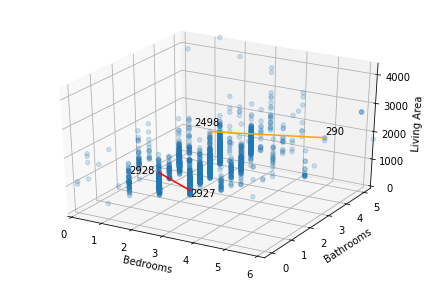
\includegraphics{closer.png}

Let's actually calculate these two distances.

    \begin{Verbatim}[commandchars=\\\{\}]
{\color{incolor}In [{\color{incolor}7}]:} \PY{c+c1}{\PYZsh{} Distance between two points connected by red line}
        \PY{n}{x} \PY{o}{=} \PY{n}{housing\PYZus{}df\PYZus{}quant}\PY{o}{.}\PY{n}{loc}\PY{p}{[}\PY{l+m+mi}{2927}\PY{p}{]}
        \PY{n}{x1} \PY{o}{=} \PY{n}{housing\PYZus{}df\PYZus{}quant}\PY{o}{.}\PY{n}{loc}\PY{p}{[}\PY{l+m+mi}{2928}\PY{p}{]}
        
        \PY{n}{np}\PY{o}{.}\PY{n}{sqrt}\PY{p}{(}\PY{p}{(}\PY{p}{(}\PY{n}{x} \PY{o}{\PYZhy{}} \PY{n}{x1}\PY{p}{)} \PY{o}{*}\PY{o}{*} \PY{l+m+mi}{2}\PY{p}{)}\PY{o}{.}\PY{n}{sum}\PY{p}{(}\PY{p}{)}\PY{p}{)}
\end{Verbatim}


\begin{Verbatim}[commandchars=\\\{\}]
{\color{outcolor}Out[{\color{outcolor}7}]:} 419.00119331572313
\end{Verbatim}
            
    \begin{Verbatim}[commandchars=\\\{\}]
{\color{incolor}In [{\color{incolor}8}]:} \PY{c+c1}{\PYZsh{} Distance between two points connected by orange line}
        \PY{n}{x} \PY{o}{=} \PY{n}{housing\PYZus{}df\PYZus{}quant}\PY{o}{.}\PY{n}{loc}\PY{p}{[}\PY{l+m+mi}{2498}\PY{p}{]}
        \PY{n}{x1} \PY{o}{=} \PY{n}{housing\PYZus{}df\PYZus{}quant}\PY{o}{.}\PY{n}{loc}\PY{p}{[}\PY{l+m+mi}{290}\PY{p}{]}
        
        \PY{n}{np}\PY{o}{.}\PY{n}{sqrt}\PY{p}{(}\PY{p}{(}\PY{p}{(}\PY{n}{x} \PY{o}{\PYZhy{}} \PY{n}{x1}\PY{p}{)} \PY{o}{*}\PY{o}{*} \PY{l+m+mi}{2}\PY{p}{)}\PY{o}{.}\PY{n}{sum}\PY{p}{(}\PY{p}{)}\PY{p}{)}
\end{Verbatim}


\begin{Verbatim}[commandchars=\\\{\}]
{\color{outcolor}Out[{\color{outcolor}8}]:} 5.0990195135927845
\end{Verbatim}
            
    Surprised by the answer? The scatterplot is deceiving because it
automatically scales the variables to make the points fit on the same
plot. In reality, the variables are on very different scales. The number
of bedrooms and bathrooms range from 0 to 6, while living area is in the
thousands. When variables are on such different scales, the variable
with the largest variability will dominate the distance metric.

The plot below shows the same data, but drawn to scale. You can see that
differences in the number of bedrooms and the number of bathrooms hardly
matter at all; only the variability in the living area matters.

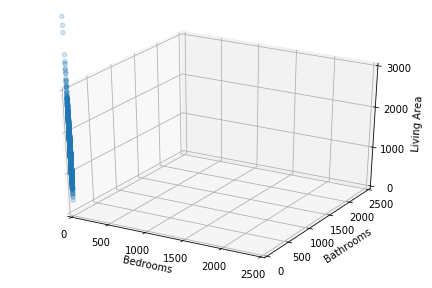
\includegraphics{closer_rescaled.png}

    To obtain distances that agree more with our intuition---and that do not
give too much weight to any one variable---we transform the variables to
be on the same scale. There are a few ways to \textbf{scale} a variable:

\begin{itemize}
\tightlist
\item
  \textbf{standardizing}: subtract each variable by its mean, then
  divide by its standard deviation,
  \[ x_i \leftarrow \frac{x_i - \text{mean}[X]}{\text{SD}[X]} \]
\item
  \textbf{normalizing}: scale each variable to have length (or ``norm'')
  1, \[ x_i \leftarrow \frac{x_i}{\sqrt{\sum_{i=1}^n x_i^2}} \]
\item
  \textbf{min/max scaling}: scale each variable so that all values are
  between 0 and 1,
  \[x_i \leftarrow \frac{x_i - \min[X]}{\max[X] - \min[X]}.\]
\end{itemize}

The figure below illustrates what each of these scaling methods do to a
synthetic data set with two variables. All three methods scale the
variables in similar (but slightly different) ways, resulting in
figure-eights with different aspect ratios. Standardizing also moves the
data to be centered around the origin, while min-max scaling moves the
data to be in a box whose corners are \((0, 0)\) and \((1, 1)\).

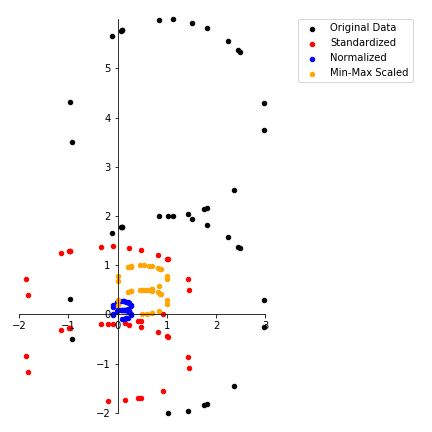
\includegraphics{scaling.png}

Let's standardize the Ames housing data, and see how it affects the
distance metric.

    \begin{Verbatim}[commandchars=\\\{\}]
{\color{incolor}In [{\color{incolor}9}]:} \PY{n}{housing\PYZus{}df\PYZus{}std} \PY{o}{=} \PY{p}{(}
            \PY{p}{(}\PY{n}{housing\PYZus{}df\PYZus{}quant} \PY{o}{\PYZhy{}} \PY{n}{housing\PYZus{}df\PYZus{}quant}\PY{o}{.}\PY{n}{mean}\PY{p}{(}\PY{p}{)}\PY{p}{)} \PY{o}{/} 
            \PY{n}{housing\PYZus{}df\PYZus{}quant}\PY{o}{.}\PY{n}{std}\PY{p}{(}\PY{p}{)}
        \PY{p}{)}
        \PY{n}{housing\PYZus{}df\PYZus{}std}
\end{Verbatim}


\begin{Verbatim}[commandchars=\\\{\}]
{\color{outcolor}Out[{\color{outcolor}9}]:}       Bedroom AbvGr  Gr Liv Area  Bathrooms
        0          0.176064     0.309212  -1.176462
        1         -1.032058    -1.194223  -1.176462
        {\ldots}             {\ldots}          {\ldots}        {\ldots}
        2928      -1.032058    -0.218968  -1.176462
        2929       0.176064     0.989715   1.156819
        
        [2930 rows x 3 columns]
\end{Verbatim}
            
    Notice that the resulting \texttt{DataFrame} contains negative values.
This makes sense because standardizing makes the mean of every variable
equal to 0. If the mean is 0, then some values must be negative.

The above command is deceptively simple. We actually subtracted a
\texttt{DataFrame} by a \texttt{Series}, then divided the resulting
\texttt{DataFrame} by another \texttt{Series}. We relied on
\texttt{pandas} to broadcast each \texttt{Series} over the right
dimension of the \texttt{DataFrame}. To be more explicit about the
broadcasting, we could have also used the \texttt{.sub()} and
\texttt{.divide()} methods (instead of \texttt{-} and \texttt{/}) and
been explicit about the axis:

    \begin{Verbatim}[commandchars=\\\{\}]
{\color{incolor}In [{\color{incolor}17}]:} \PY{n}{housing\PYZus{}df\PYZus{}std} \PY{o}{=} \PY{p}{(}\PY{n}{housing\PYZus{}df\PYZus{}quant}\PY{o}{.}
                           \PY{n}{sub}\PY{p}{(}\PY{n}{housing\PYZus{}df\PYZus{}quant}\PY{o}{.}\PY{n}{mean}\PY{p}{(}\PY{p}{)}\PY{p}{,} \PY{n}{axis}\PY{o}{=}\PY{l+m+mi}{1}\PY{p}{)}\PY{o}{.}
                           \PY{n}{divide}\PY{p}{(}\PY{n}{housing\PYZus{}df\PYZus{}quant}\PY{o}{.}\PY{n}{std}\PY{p}{(}\PY{p}{)}\PY{p}{,} \PY{n}{axis}\PY{o}{=}\PY{l+m+mi}{1}\PY{p}{)}\PY{p}{)}
         \PY{n}{housing\PYZus{}df\PYZus{}std}
\end{Verbatim}


\begin{Verbatim}[commandchars=\\\{\}]
{\color{outcolor}Out[{\color{outcolor}17}]:}       Bedroom AbvGr  Gr Liv Area  Bathrooms
         0          0.176064     0.309212  -1.176462
         1         -1.032058    -1.194223  -1.176462
         {\ldots}             {\ldots}          {\ldots}        {\ldots}
         2928      -1.032058    -0.218968  -1.176462
         2929       0.176064     0.989715   1.156819
         
         [2930 rows x 3 columns]
\end{Verbatim}
            
    Now let's recalculate the distances using this standardized data and see
if our conclusions change.

    \begin{Verbatim}[commandchars=\\\{\}]
{\color{incolor}In [{\color{incolor}11}]:} \PY{c+c1}{\PYZsh{} Distance between two points connected by red line}
         \PY{n}{x} \PY{o}{=} \PY{n}{housing\PYZus{}df\PYZus{}std}\PY{o}{.}\PY{n}{loc}\PY{p}{[}\PY{l+m+mi}{2927}\PY{p}{]}
         \PY{n}{x1} \PY{o}{=} \PY{n}{housing\PYZus{}df\PYZus{}std}\PY{o}{.}\PY{n}{loc}\PY{p}{[}\PY{l+m+mi}{2928}\PY{p}{]}
         
         \PY{n}{np}\PY{o}{.}\PY{n}{sqrt}\PY{p}{(}\PY{p}{(}\PY{p}{(}\PY{n}{x} \PY{o}{\PYZhy{}} \PY{n}{x1}\PY{p}{)} \PY{o}{*}\PY{o}{*} \PY{l+m+mi}{2}\PY{p}{)}\PY{o}{.}\PY{n}{sum}\PY{p}{(}\PY{p}{)}\PY{p}{)}
\end{Verbatim}


\begin{Verbatim}[commandchars=\\\{\}]
{\color{outcolor}Out[{\color{outcolor}11}]:} 1.4651211129695825
\end{Verbatim}
            
    \begin{Verbatim}[commandchars=\\\{\}]
{\color{incolor}In [{\color{incolor}12}]:} \PY{c+c1}{\PYZsh{} Distance between two points connected by orange line}
         \PY{n}{x} \PY{o}{=} \PY{n}{housing\PYZus{}df\PYZus{}std}\PY{o}{.}\PY{n}{loc}\PY{p}{[}\PY{l+m+mi}{2498}\PY{p}{]}
         \PY{n}{x1} \PY{o}{=} \PY{n}{housing\PYZus{}df\PYZus{}std}\PY{o}{.}\PY{n}{loc}\PY{p}{[}\PY{l+m+mi}{290}\PY{p}{]}
         
         \PY{n}{np}\PY{o}{.}\PY{n}{sqrt}\PY{p}{(}\PY{p}{(}\PY{p}{(}\PY{n}{x} \PY{o}{\PYZhy{}} \PY{n}{x1}\PY{p}{)} \PY{o}{*}\PY{o}{*} \PY{l+m+mi}{2}\PY{p}{)}\PY{o}{.}\PY{n}{sum}\PY{p}{(}\PY{p}{)}\PY{p}{)}
\end{Verbatim}


\begin{Verbatim}[commandchars=\\\{\}]
{\color{outcolor}Out[{\color{outcolor}12}]:} 3.9440754446060033
\end{Verbatim}
            
    So, if we first standardize the data, then the pair of observations
connected by the red line are more similar than the pair connected by
the orange line, which matches our intuition. It is (almost) always a
good idea to scale your variables before calculating distances.

Now that you've seen how to implement one scaling method
(standardization), you will implement two more (normalization and
min-max scaling) in Exercises 1 and 2 below.

    \hypertarget{exercises}{%
\section{Exercises}\label{exercises}}

    \textbf{Exercise 1.} Instead of standardizing the three variables from
the Ames housing data set, normalize them. Then, recompute the distances
between the two pairs of points above. Does your conclusion change?

    \begin{Verbatim}[commandchars=\\\{\}]
{\color{incolor}In [{\color{incolor}36}]:} \PY{c+c1}{\PYZsh{} YOUR CODE HERE}
         \PY{c+c1}{\PYZsh{} BEGIN SOLUTION}
         \PY{n}{housing\PYZus{}df\PYZus{}norm} \PY{o}{=} \PY{p}{(}\PY{n}{housing\PYZus{}df\PYZus{}quant}\PY{o}{.}
                           \PY{n}{divide}\PY{p}{(}\PY{n}{np}\PY{o}{.}\PY{n}{sqrt}\PY{p}{(}\PY{p}{(}\PY{n}{housing\PYZus{}df\PYZus{}quant}\PY{o}{*}\PY{o}{*}\PY{l+m+mi}{2}\PY{p}{)}\PY{o}{.}\PY{n}{sum}\PY{p}{(}\PY{n}{axis}\PY{o}{=}\PY{l+m+mi}{0}\PY{p}{)}\PY{p}{)}\PY{p}{,} \PY{n}{axis}\PY{o}{=}\PY{l+m+mi}{1}\PY{p}{)}\PY{p}{)}
         \PY{n}{display}\PY{p}{(}\PY{n}{housing\PYZus{}df\PYZus{}norm}\PY{p}{)}
         \PY{n}{x} \PY{o}{=} \PY{n}{housing\PYZus{}df\PYZus{}norm}\PY{o}{.}\PY{n}{loc}\PY{p}{[}\PY{l+m+mi}{2927}\PY{p}{]}
         \PY{n}{x1} \PY{o}{=} \PY{n}{housing\PYZus{}df\PYZus{}norm}\PY{o}{.}\PY{n}{loc}\PY{p}{[}\PY{l+m+mi}{2928}\PY{p}{]}
         
         \PY{n}{display}\PY{p}{(}\PY{n}{np}\PY{o}{.}\PY{n}{sqrt}\PY{p}{(}\PY{p}{(}\PY{p}{(}\PY{n}{x} \PY{o}{\PYZhy{}} \PY{n}{x1}\PY{p}{)} \PY{o}{*}\PY{o}{*} \PY{l+m+mi}{2}\PY{p}{)}\PY{o}{.}\PY{n}{sum}\PY{p}{(}\PY{p}{)}\PY{p}{)}\PY{p}{)}
         
         \PY{n}{x} \PY{o}{=} \PY{n}{housing\PYZus{}df\PYZus{}norm}\PY{o}{.}\PY{n}{loc}\PY{p}{[}\PY{l+m+mi}{2498}\PY{p}{]}
         \PY{n}{x1} \PY{o}{=} \PY{n}{housing\PYZus{}df\PYZus{}norm}\PY{o}{.}\PY{n}{loc}\PY{p}{[}\PY{l+m+mi}{290}\PY{p}{]}
         
         \PY{n}{np}\PY{o}{.}\PY{n}{sqrt}\PY{p}{(}\PY{p}{(}\PY{p}{(}\PY{n}{x} \PY{o}{\PYZhy{}} \PY{n}{x1}\PY{p}{)} \PY{o}{*}\PY{o}{*} \PY{l+m+mi}{2}\PY{p}{)}\PY{o}{.}\PY{n}{sum}\PY{p}{(}\PY{p}{)}\PY{p}{)}
         \PY{n+nb}{print}\PY{p}{(}\PY{l+s+s2}{\PYZdq{}}\PY{l+s+s2}{In this case, the conclusion is about the same}\PY{l+s+s2}{\PYZdq{}}\PY{p}{)}
         \PY{c+c1}{\PYZsh{} END SOLUTION}
\end{Verbatim}


    
    \begin{verbatim}
      Bedroom AbvGr  Gr Liv Area  Bathrooms
0          0.018649     0.019331   0.009878
1          0.012433     0.010460   0.009878
...             ...          ...        ...
2928       0.012433     0.016215   0.009878
2929       0.018649     0.023347   0.024695

[2930 rows x 3 columns]
    \end{verbatim}

    
    
    \begin{verbatim}
0.0079100215088419978
    \end{verbatim}

    
    \begin{Verbatim}[commandchars=\\\{\}]
In this case, the conclusion is about the same

    \end{Verbatim}

    \textbf{Exercise 2.} Instead of standardizing the three variables from
the Ames housing data set, apply a min-max scaling to them. Then,
recompute the distances between the two pairs of points above. Does your
conclusion change?

    \begin{Verbatim}[commandchars=\\\{\}]
{\color{incolor}In [{\color{incolor} }]:} \PY{c+c1}{\PYZsh{} YOUR CODE HERE}
\end{Verbatim}


    Exercises 3-5 ask you to work with a data set that describes the
chemical composition of 1599 red wines
(\texttt{https://raw.githubusercontent.com/dlsun/data-science-book/master/data/wines/reds.csv}).
There are 12 variables in this data set, all of which are quantitative
(so each observation is a point in 12-dimensional space).

    \textbf{Exercise 3.} Which red wine is more similar to wine 0 in the
\texttt{DataFrame}: wine 6 or wine 36? (Do not scale the variables.)
Does your answer depend on which distance metric you use to measure
``similarity''?

    \begin{Verbatim}[commandchars=\\\{\}]
{\color{incolor}In [{\color{incolor} }]:} \PY{c+c1}{\PYZsh{} YOUR CODE HERE}
\end{Verbatim}


    \textbf{Exercise 4.} Now suppose we agree to measure similarity using
Euclidean distance, and we wish to investigate the effect of scaling the
variables. Which red wine is more similar to wine 0: wine 6 or wine 36?
Does the answer depend on whether the variables are scaled or not? Does
it depend on the choice of scaling?

    \begin{Verbatim}[commandchars=\\\{\}]
{\color{incolor}In [{\color{incolor} }]:} \PY{c+c1}{\PYZsh{} YOUR CODE HERE}
\end{Verbatim}


    \textbf{Exercise 5.} Which wine is most similar to wine 267? Try
different distance metrics and different scaling methods. How sensitive
is your conclusion to the choice of distance metric and scaling method?

\emph{Hint:} You can do this without a \texttt{for} loop. Take advantage
of broadcasting!

    \begin{Verbatim}[commandchars=\\\{\}]
{\color{incolor}In [{\color{incolor} }]:} \PY{c+c1}{\PYZsh{} YOUR CODE HERE}
\end{Verbatim}



    % Add a bibliography block to the postdoc
    
    
    
    \end{document}
